\documentclass[tikz,border=2pt]{standalone}
\usetikzlibrary{decorations.pathmorphing,decorations.pathreplacing}
\usetikzlibrary{calc}
\usetikzlibrary{arrows.meta}
\usepackage{bm}

\begin{document}
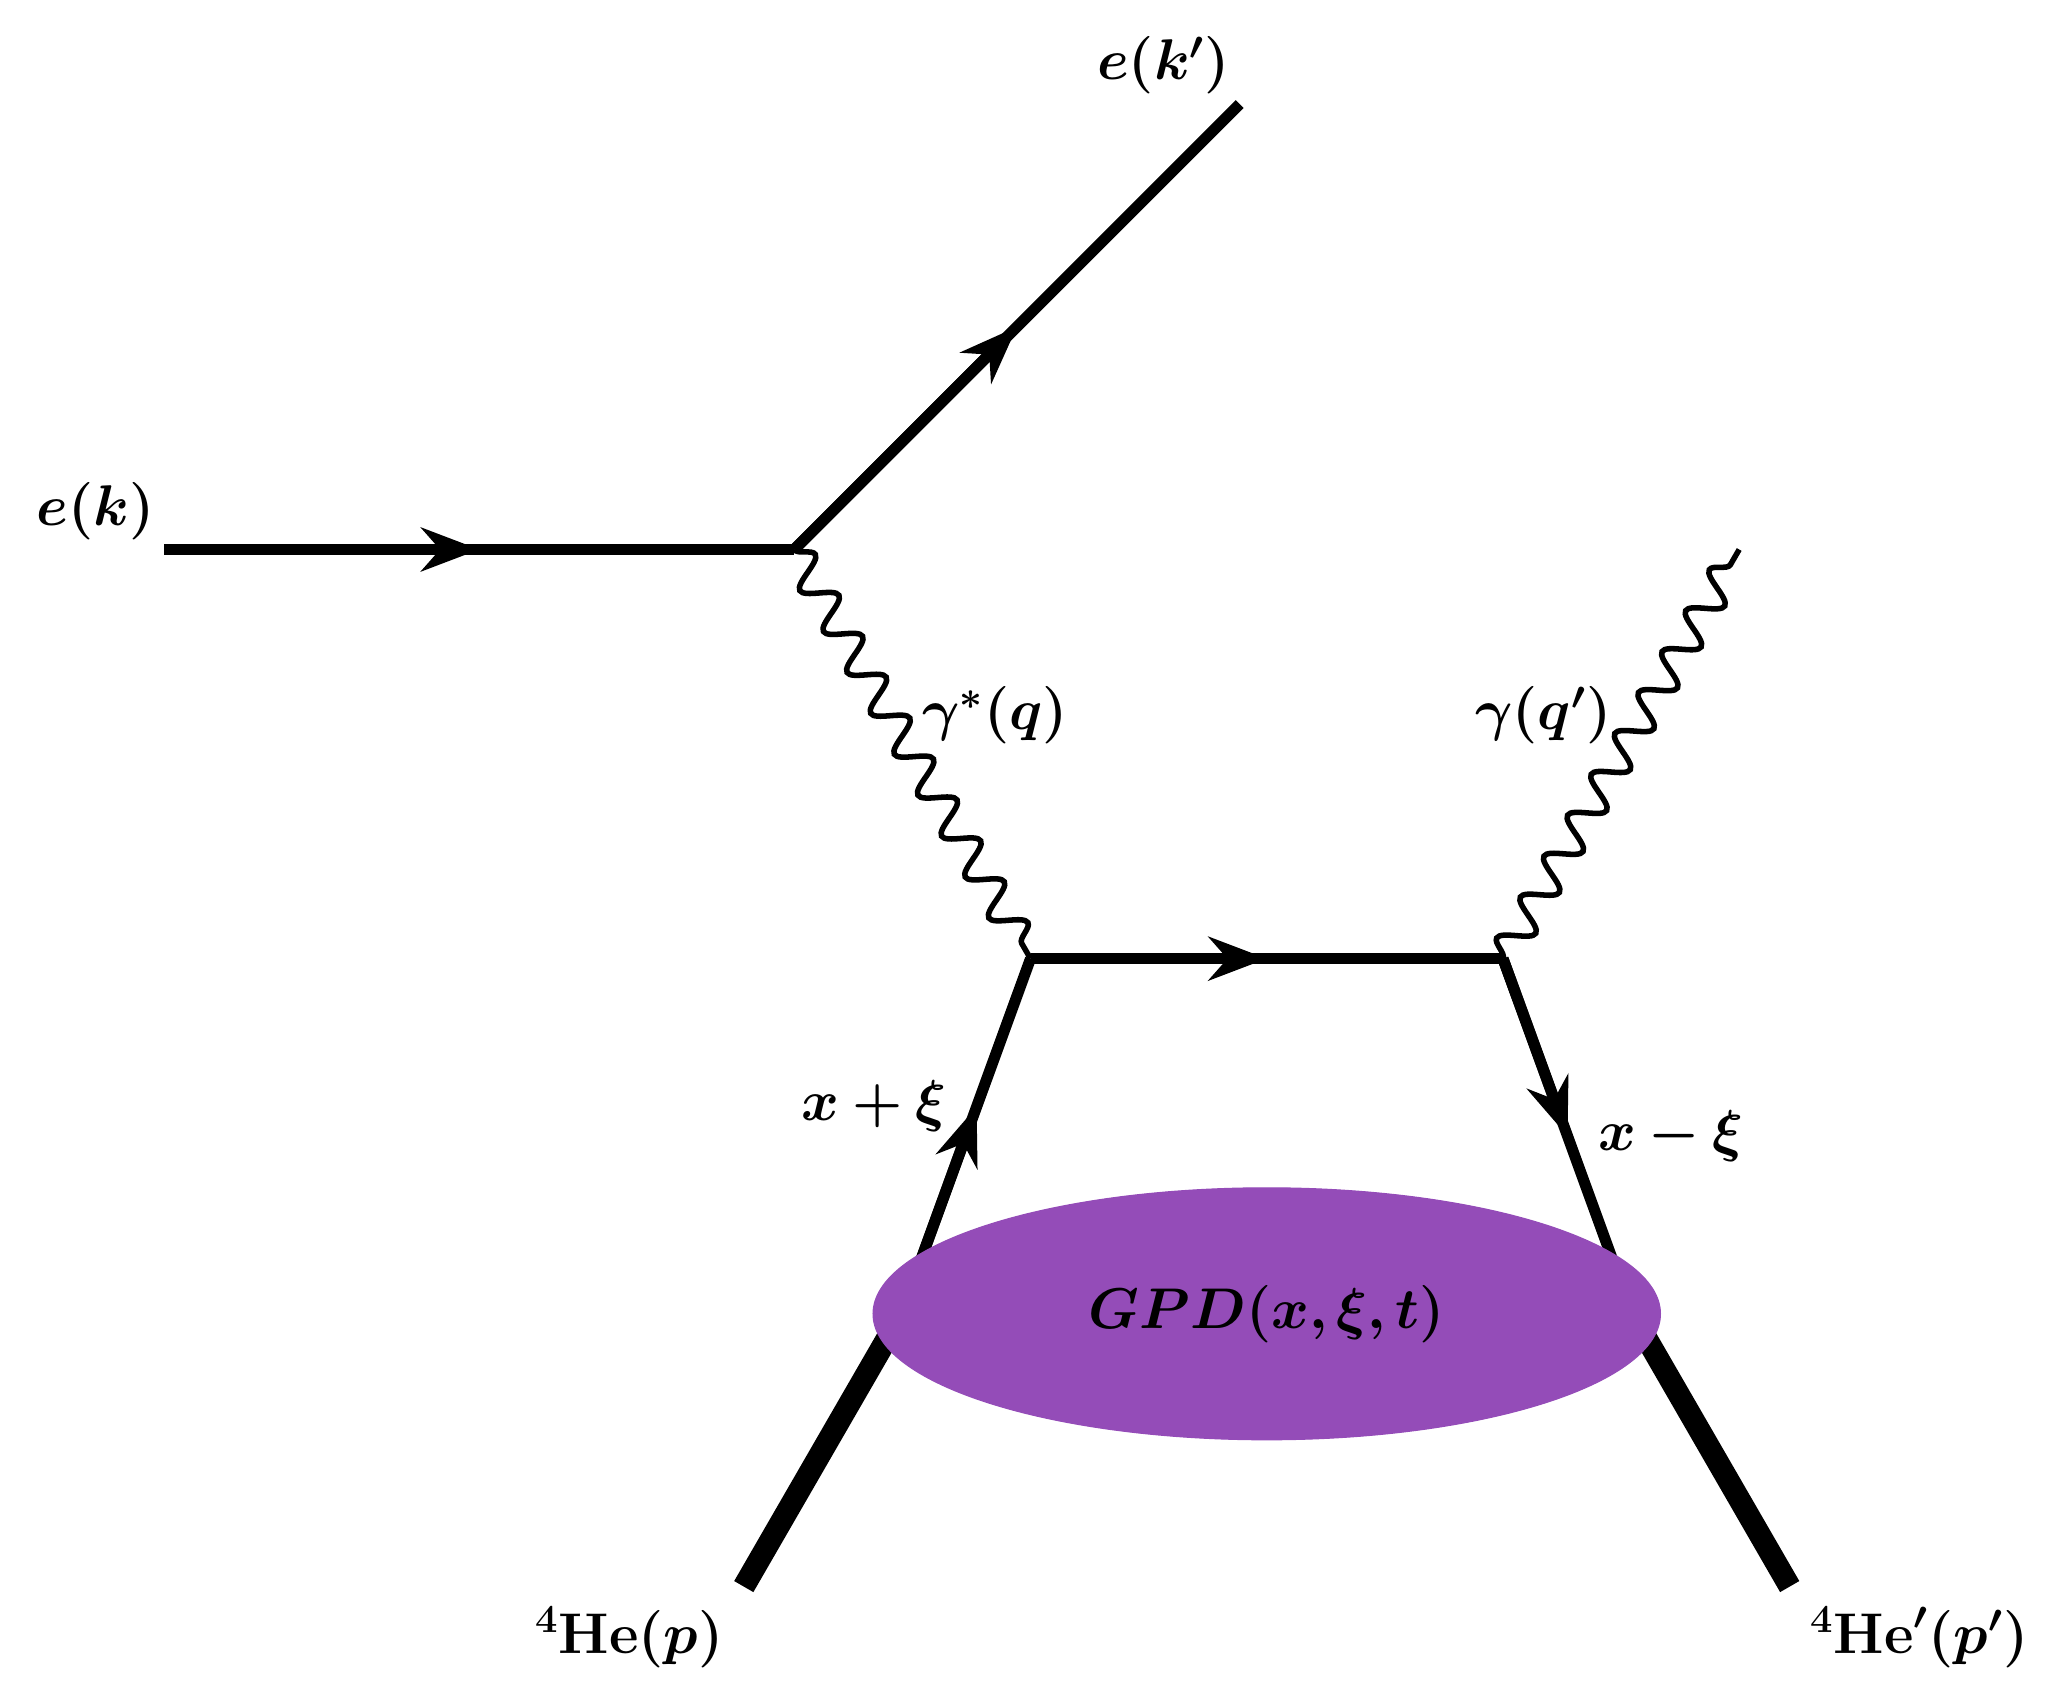
\begin{tikzpicture}[scale=4]
    % incoming electron
    \draw [very thick, line width=4pt] (-2,0) -- (0,0);
    \draw [very thick, line width=4pt, -{Stealth}] (-2,0) -- (-1,0);
    \node [above left] at (-2,0) {\huge $\bm{e(k)}$};
    % scattered electron
    \draw [very thick, line width=4pt] (0,0) -- (45:2);
    \draw [very thick, line width=4pt, -{Stealth}] (0,0) -- (45:1);
    \node [above left] at (45:2) {\huge $\bm{e(k^\prime)}$};
    % virtual photon
    \draw[decorate, decoration={snake,  amplitude=2mm, segment length=6mm}, very thick, line width=2pt] (0,0) -- (-60:1.5);
    \node [above right] at (-60:0.75) {\huge \bm{$\gamma^*(q)}$};
    % incoming and outgoing quarks
    \draw [very thick, line width=4pt] (-60:1.5) -- ++(-110:1.2);
        \draw [very thick, line width=4pt, -{Stealth}] (-60:1.5) ++(-110:1.2) -- ++(70:0.7) node [left] {\huge $\bm{x+\xi}\;$};
    \draw [very thick, line width=4pt] (-60:1.5) -- ++(1.5,0);
        \draw [very thick, line width=4pt, -{Stealth}] (-60:1.5) -- ++(0.75,0);
    \draw [very thick, line width=4pt] (-60:1.5) ++(1.5,0) -- ++(-70:1.2);
        \draw [very thick, line width=4pt, -{Stealth}] (-60:1.5)  ++(1.5,0) -- ++(-70:0.6) node [right] {\huge $\;\bm{x-\xi}$};
    % produced photon
    \draw[decorate, decoration={snake,  amplitude=2mm, segment length=6mm}, very thick, line width=2pt] (-60:1.5) ++(1.5,0) -- ++(60:1.5);
    \path (-60:1.5) ++(1.5,0) ++(60:0.75) node [above left] {\huge $\bm{\gamma(q^\prime)}$};
    % GPD
    \coordinate (A) at ($(-60:1.5) + (-110:1.2)$);
    \coordinate (B) at ($(-60:1.5) + (1.5,0) +(-70:1.2)$);
    \coordinate (M) at ($(A)!0.5!(B)$);
    %\node [below] at (A) {A};
    %\node [below] at (B) {B};
    % fixed target
    \draw [very thick, line width=8pt] (A) -- ++(-120:1) node [below left] {\huge $\bm{^4\mbox{He}(p)}$};
    % recoil fragment
    \draw [very thick, line width=8pt] (B) -- ++(-60:1) node [below right] {\huge $\bm{^4\mbox{He}^\prime(p^\prime)}$};
    % GPD text
    \filldraw [blue!60!red!70] (M) ellipse (1.25 and 0.4);
    \node at (M) {\huge $\bm{GPD(x, \xi, t)}$};
    

    % % target as circle
    % \draw [very thick] (0,-2) circle [radius=0.5];
    % % incomming target
    % \draw [very thick, line width=4pt] (0,-2) ++(210:0.5) -- ++(210:2);
    % \draw [very thick, line width=4pt, -{Stealth}] (0,-2) ++(210:2.5) -- ++(210+180:1);
    % \node [above left] at ($(0,-2)+(210:1.5)$) {\huge $p(p_1)$};
    % % outgoing target
    % \draw [very thick, line width=4pt] (0,-2) ++(-30:0.5) -- ++(-30:2);
    % \draw [very thick, line width=4pt, -{Stealth}] (0,-2) ++(-30:0.5) -- ++(-30:1);
    % \node [above right] at ($(0,-2)+(-30:1.5)$) {\huge $p(p_2)$};


\end{tikzpicture}
\end{document}